\section{Iteration \#1 -- Pseudo-Pyramid Tree}

TODO: iteration summary

\subsection{Defragmented and Rebuild Pseudo-Pyramid Tree}

\begin{wrapfigure}[12]{r}{0.5\textwidth}
	\vspace{-40pt}
	\begin{center}
		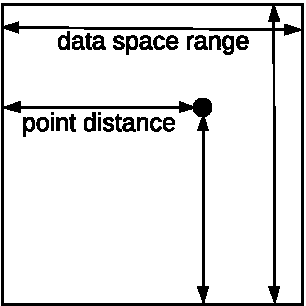
\includegraphics[scale=0.6]{figures/pseudo-pyramid_tree_point_boundary_distances.pdf}
	\end{center}
	\vspace{-20pt}
	\caption{Computing Distance of Point Along Pseudo-Pyramid Tree Boundary Along Each Dimension}
	\label{fig:point-boundary-distance}
\end{wrapfigure}

The School of Computing have an implementation of an index structure which is similar to the Pyramid tree, originally written by Zhao Geng\footnote{Z.Geng@leeds.ac.uk}. All the points are stored in a single \texttt{std::vector}. Each point is hashed to an integer representation which acts as the key to a bucket stored in a hash map (specifically \texttt{boost::unordered\_map}, part of the Boost\footnote{\url{http://www.boost.org/}} library). A bucket is a \texttt{std::vector} that contains indices to points in the large point array.

To determine if a point $p$ is stored in the structure, $p$ is first hashed into its one-dimensional representation. The corresponding bucket is then sequentially scanned until the point is found or the end of the bucket is reached. To reduce the number of floating point comparisons, especially for large $d$, the \textit{sums} of each point are stored when they are inserted. This way, a $O(d)$ point comparison needs to be made if the $O(1)$ point sum comparison passes. Simple optimisations were initially made to the original implementation. The original implementation passed many heap allocated structures by-value, resulting in excessive copies and more time being spent allocating memory and copying data. These copies were not necessary and were removed where possible by passing the data by-reference.

In this report, this implementation shall be called the \textbf{Pseudo-Pyramid Tree}. This is because the hashing function used is \textit{inspired} by the Pyramid tree, but is not the same\footnote{There is code to compute the pyramid value of a point in the original code, but curiously it is not used when inserting or querying points. An alternative hashing function was used instead.}. Let $min_i$ and $max_i$ define the minimum and maximum bounds for dimension $i$ and $p$ be a point. To hash $p$, how far along the boundary $p$ is in each dimension is computed using Equation \ref{eq:point-boundary-distance} first. See Figure \ref{fig:point-boundary-distance} for an illustration of what these values mean.

\begin{equation}
	h_i(p) = \frac{p_i - min_i}{max_i - min_i}
	\label{eq:point-boundary-distance}
\end{equation}

Let $B$ be a parameter which controls how likely points will be in the same bucket and let $m$ be a point where $m_i = \ceil{B^{\frac{1}{d}}}$ for $0 \leq i \leq d$. The hashed value $h(p)$ of a point $p$ is then given by Equation \ref{eq:pseudo-pyramid-hash},  where \texttt{toInt} converts a real number to an integer by truncating the decimal part. Computing this is a $O(d^2)$ operation due to the inner loop to compute $\prod_{j=0}^{i}{\lbrack m_j \rbrack}$.

\begin{equation}
	h(p) = \sum_{i = 0}^{d} { \lbrack \texttt{toInt}( h_i(p) \times m_i ) \times \prod_{j=0}^{i}{\lbrack m_j \rbrack} \rbrack }
	\label{eq:pseudo-pyramid-hash}
\end{equation}

Higher $B$ means higher $m$. This increases the magnitude of $h_i(p)$ before it is truncated to an integer, meaning less points will have the same hashed value, meaning less points in the same bucket on average. Lower $B$ will therefore mean more points will be in the same bucket on average.

The original implementation of the Pseudo-Pyramid Tree did not provide \texttt{delete} and \texttt{update} operations, meaning a \texttt{delete} procedure had to be added. To delete a point $p$, the point is first hashed and the bucket containing the point is found. The index pointing to $p$ in the bucket is removed from the bucket, but the actual point itself is not removed the point array. In other words, the memory is never released until the whole structure is deleted. This makes the structure useful for batch computation because it can be discarded straight after a task, releasing all allocated memory then. However, if the structure is used as part of a long-running process then this is not suitable because there is the potential to run out of memory. This will be referred to as the \textbf{Batch Pseudo-Pyramid Tree} for the rest of this document.

Variants of this structure were implemented to provide a \texttt{delete} operation. The first is the \textbf{Defragmented Pseudo-Pyramid Tree}. When a point's index is deleted from a bucket, the element at the index is marked for deletion from the array at a later time (by adding the index of the point to another \texttt{std::vector}). If the number of marked elements exceeds a certain number $R$, then the $R + 1$ marked elements are erased from the vector (i.e. memory is released). The indices in each bucket are then updated to point to the correct element in the modified array. Even though \texttt{delete} is normally a constant time operation, the worst case is $O(n^2)$ because of this defragmentation procedure.

The \textbf{Rebuild Pseudo-Pyramid Tree} uses a different strategy for releasing memory for unused points. Instead of defragmenting the array by peforming a sequence of array deletions when $R + 1$ elements are marked for deletion, the entire structure is rebuilt. This new cleanup procedure starts by clearing the structure and incrementally building the new structure by only adding points \textit{not} marked for deletion. $n - R$ points will be re-instered and insertion in the worst case is $O(n)$, meaning the worst case complexity of \texttt{delete} is $O((n - R)n)$. The larger $R$ is, the less time it takes to perform this procedure but a larger amount of allocated memory goes unused at a time.

\subsection{Accelerating Hash Function}

TODO: rearrange
It was shown in the last iteration that the Pseudo-Pyramid tree eventually becomes slower than Sequential Scan as $d$ increases. Since the plots showed the increase in the Pseudo-Pyramid Tree's execution time is roughly quadratic, and the structure spend most of that time in the $O(d^2)$ hashing function (Equation \ref{eq:pseudo-pyramid-hash}), it follows that speeding up the hashing function would provide large speed gains.

The existing point hashing function takes $O(d^2)$ time because of the inner loop that computes $\prod_{j=0}^{i}{\lbrack m_j \rbrack}$. If $m$ is changed during the structure's lifetime. otherwise the hash value of a point could change and stored points can become inaccessible. Therefore, $m$ is constant and the hashing function can computed in $O(d)$ time by \textit{pre-computing} $\prod_{j=0}^{i}{\lbrack m_j \rbrack}$. This pre-computation happens when the Pseudo-Pyramid tree is initialised. The new hashing function is given in Equation \ref{eq:new-pseudo-pyramid-hash}.

\begin{multline}\\
	h(p) = \sum_{i = 0}^{d} { \lbrack \texttt{toInt}( h_i(p) \times m_i ) \times M_i \rbrack } \\
	\text{where } M_i = \prod_{j=0}^{i}{\lbrack m_j \rbrack} \;\;\; \text{for} \; 0 \leq i \leq d \\
	\label{eq:new-pseudo-pyramid-hash}
\end{multline}

Table \ref{tab:new-pseudo-pyramid-hash} shows operation execution time of the Batch Pyramid Tree using the original $O(d^2)$ hashing function and the new $O(d)$ function. The test used the Insert-Query-Remove operation list on the uniform synthetic dataset with 200 dimensions. Figure \ref{fig:new-pseudo-pyramid-hash} plots the performance of the Pseudo-Pyramid tree with both hash functions alongside Sequential Scan, showing execution time against dimensionality. From the plot, it is clear that the new hashing function provides superior speed; the Pseudo-Pyramid Tree is now significantly faster than Sequential Scan, even for dimensions as high as 200.

\begin{table}
	\centering
	\begin{tabular}{|l|l|l|}
		\hline
		\textbf{Operation} & \textbf{$O(d^2)$ Function} & \textbf{$O(d)$ Function} \\
		\hline
		\textbf{Insert} & 1.46412 & 0.0112199 \\
		\textbf{Delete} & 0.730777 & 0.00625336 \\
		\textbf{Point Query} & 0.731469 & 0.0076015 \\
		\hline
	\end{tabular}
	\caption{Total Execution Time (in Seconds) of Batch Pseudo-Pyramid Tree Using $O(d^2)$ and $O(d)$ Hash Function (200D Randomly Uniform Dataset, 10,000 operations each)}
	\label{tab:new-pseudo-pyramid-hash}
\end{table}

\begin{figure}
	\centering
	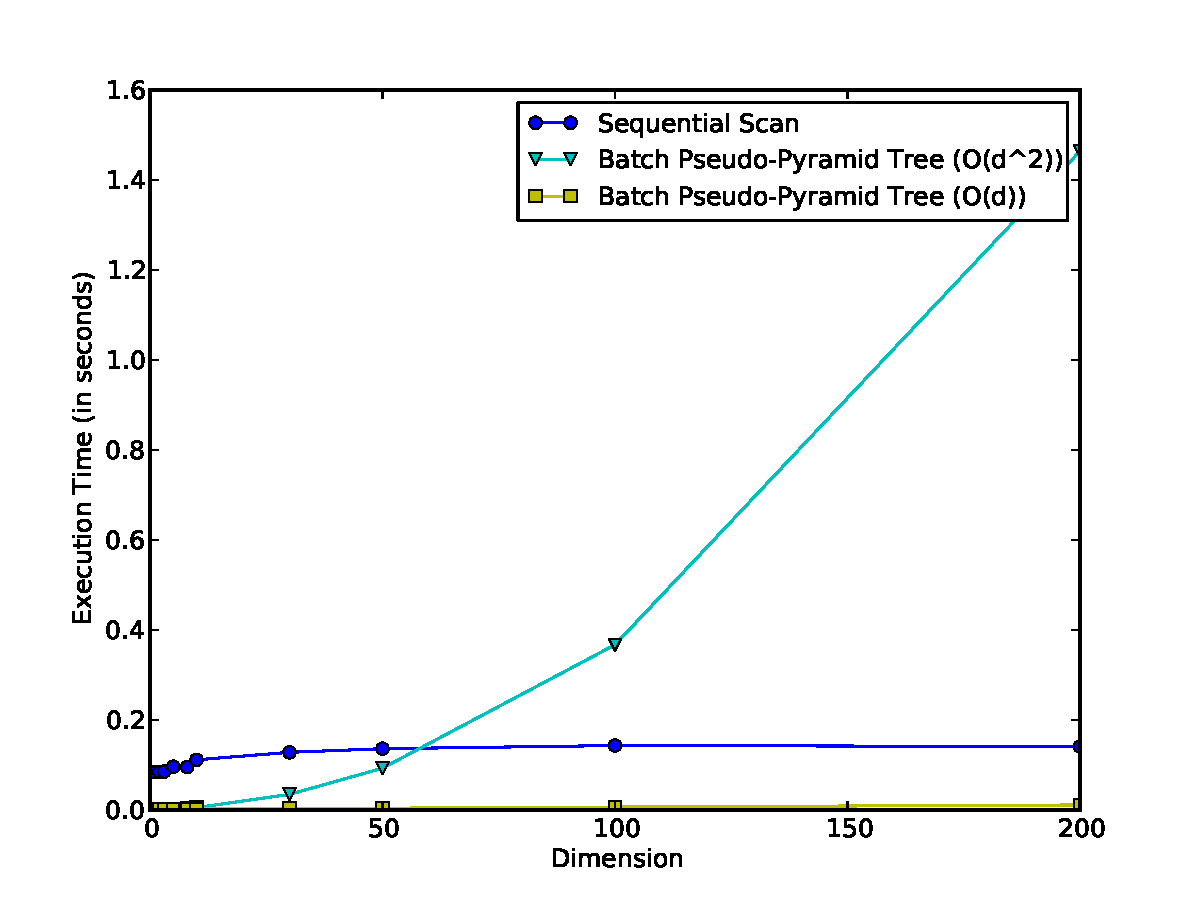
\includegraphics[scale=0.5]{figures/performance_analysis/iteration_2/new_pseudo-pyramid_hash_performance.pdf}
	\caption{\texttt{insert} Performance on Random Uniformly Distributed Datasets of Varying Dimensions}
	\label{fig:new-pseudo-pyramid-hash}
\end{figure}

\subsection{Bucket Pseudo-Pyramid Tree}

The Bucket Pseudo-Pyramid Tree implementation does not use a single array to store the points. Instead of buckets containing an array of point indices, it has an array of actual points. No clenaup procedure is necessary because the memory for a point is released immediately afer it's removed, by simply erasing it from the corresponding bucket's array. The goal of this is to increase \textbf{cache coherency} when searhcing a bucket, since the point array can be searched sequentially. The index-based variants cause random accesses in the single point array (causing more cache misses) since a bucket's store indices may point to distant parts of the point array, which may become very large.

% TODO: further explanation of cache misses?

Array deletion is a $O(n)$ operation since the case where a single bucket stores all $n$ points is possible, making \texttt{delete} $O(n)$ in the worst case. Since the order the points are stored in a bucket do not matter, the C++ \textit{erase-remove} idiom has been used to delete elements from the bucket arrays, which swaps the element to delete with the last element in the array, removing the desired element when it's at the end of the array. This prevents the required $O(n)$ shift operation which tightly pack the elements after a deletion. From this point in the document onwards, all \texttt{std::vector} deletions where order does not matter will be performed using the erase-remove idiom.

\subsection{Splay Pseudo-Pyramid Tree}

Unlile the other implementations, the Splay Pseudo-Pyramid Tree does not use a hash map as the underyling one-dimensional index structure, but a splay tree. The splay tree is a self-adjusting variant of the binary search tree that uses a \textit{splaying} operation (a heuristic) to allow faster access to recently accessed elements. \cite{splay-tree}. The splaying operation achieves this by performing a series of tree rotations that move a given node up to the root of the tree. Through amortised analysis and empirical experiments, it has been shown splay trees can be more efficient than standard binary trees for a series of non-random operations \cite{splay-tree}, despite the asymptotic worst case bound being worse than binary search trees.

TODO: more detail about the splay tree, including in-depth algorithms??

Nodes in the Splay Pseudo-Pyramid Tree correspond to individual buckets in the Bucket Pseudo-Pyramid Tree, meaning each node can store multiple points. Since the splay tree is implemented as a collection of heap-allocated nodes with pointers to link them, deletions are cheap as a low amount of memory needs to be de-allocated per \texttt{delete} operation. The aim is that this, combined with the self-adjusting nature of the splay tree, will produce a Pseudo-Pyramid Tree implementation that is more efficient for non-random operations used in real applications.

\subsection{Best Pseudo-Pyramid Tree Variant}

All variants of the Pseudo-Pyramid Tree hash $d$-dimensional points to a one-dimensional value, which is used as a key to search for a given point in a one-dimensional structure. What varies is how points are deleted and which underyling one-dimensional structure is used. The Defragmented Pseudo-Pyramid Tree is clearly inferior to the Rebuild Pseudo-Pyramid Tree from the last iteration and the Batch Pseudo-Pyramid Tree never releases memory after points are removed. For dynamic data which changes frequently, this may cause the machine to run out of memory. As such, both of these structures will not be explored further.

% TODO: create new plot
\begin{wrapfigure}[12]{r}{0.5\textwidth}
	\vspace{-40pt}
	\begin{center}
		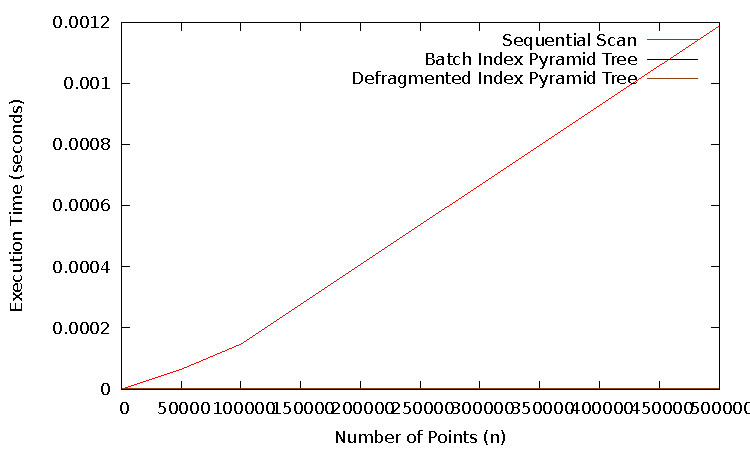
\includegraphics[scale=0.5]{figures/performance_analysis/iteration_1/all_pquery_sizevary_average.pdf}
	\end{center}
	\vspace{-20pt}
	\caption{Total Execution Time (in Seconds) of \texttt{delete} Operation for Different Sample Sizes of Astrophysics Dataset}
	\label{fig:perf2-astrophysics-delete}
\end{wrapfigure}

The Rebuild Pseudo-Pyramid Tree, Bucket Pyramid-Tree and the Splay Pseudo-Pyramid Tree were timed with the full collection of synthetic and real datasets. The results were consistent throughout the different datasets. For brevity, only the times for the astrophysics dataset with the Insert-Query-Delete operation list will be provided. Table \ref{tab:perf2-astrophysic} shows the total execution times of each structure operation and Figure \ref{fig:perf2-astrophysics-delete} shows execution time of the \texttt{delete} operation as the number of points are increased.

The results show that storing separate point arrays for each bucket drastically reduces the speed of \texttt{delete} operations, with the Rebuuild Pseudo-Pyramid tree being slowest. The differences in speed between the bucket and splay variants is small, but the Bucket Pseudo-Pyramid Tree outperforms the Splay Tree with most datasets. With severely skewed synthetic data, the splay variant is \texttt{slightly} faster, but the speed increase is neglible. This could be an indication that self-adjusting structures are useful for heavily skewed data however, highlighting an area for further study. Based on these results, it was decided that any future variants of the tree will be based on the Bucket Pseudo-Pyramid Tree.

\begin{table}
	\centering
	\begin{tabular}{|r|l|l|l|l|}
		\hline
		\textbf{Structure} & \textbf{Operation List} & $n = 10,000$ & $n = 100,000$ & $n = 500,000$ \\
		\multirow{ 4}{*}{\textbf{Defragmented Pseudo-Pyramid Tree}} & \textbf{Insert} & TODO & TODO & TODO \\
		 & \textbf{Delete} & TODO & TODO & TODO \\
		 & \textbf{Point Queries} & TODO & TODO & TODO \\		
		\hline
		\multirow{ 4}{*}{\textbf{Rebuild Pseudo-Pyramid Tree}} & \textbf{Insert} & 0.0698843 & 5.99686 & 156.281 \\
		 & \textbf{Delete} & 0.481668 & 59.3513 & 1328.2 \\
		 & \textbf{Point Queries} & 0.0656809 & 5.96501 & 158.955 \\
		\hline
		\multirow{ 4}{*}{\textbf{Bucket Pseudo-Pyramid Tree}} & \textbf{Insert} & 0.0508634 & 4.5737 & 101.581 \\
		 & \textbf{Delete} & 0.318228 & 29.4124 & 672.372 \\
		 & \textbf{Point Queries} & 0.0495212 & 4.43291 & 96.1636 \\
		\hline
		\multirow{ 4}{*}{\textbf{Splay Pseudo-Pyramid Tree}} & \textbf{Insert} & 0.0509274 & 4.64242 & 101.245 \\
		 & \textbf{Delete} & 0.318251 & 29.6108 & 675.695 \\
		 & \textbf{Point Queries} & 0.0507686 & 4.59311 & 99.1579 \\
		\hline
	\end{tabular}
	\caption{Total Execution Time (in Seconds) for Different Sample Sizes of Astrophysics Dataset using the Insert-Query-Delete Operation List}
	\label{tab:perf2-astrophysics}
\end{table}

\subsection{Performance Timings}

TODO: flesh out with additinoal structyures

The structures being analysed in this iteration are sequential scan, octree and the pseudo-pyramid trees (batch and defragmented). $B = 300000$ and $R=3000$ was used as parameters for the Pseudo-Pyramid Trees. This means the Defagmented Pseudo-Pyramid Tree defragments when 3001 elements have been marked for deletion. Table \ref{tab:perf1-randuniform} contains the \textit{total} runtime of \texttt{insert}, \texttt{delete} and point query for uniformly randomly generated points for the analysed structures. When ``-" is shown instead of the number of seconds, it means that the performance test could not finish due to the machine running out of memory. Plots with dimension against execution time are shown for the three operations in Figures \ref{fig:perf1-allinsert-d}, \ref{fig:perf1-alldelete-d} and \ref{fig:perf1-allpquery-d}. The execution times for skewed and clustered data was almost identical to the uniformly random datasets; for the sake of brevity, the tables and plots for these datasets have been placed in Appendix \ref{chap:supp-material}. 

The three plots show that dimensionality has little effect on \textit{insert} and point queries for Sequential Scan. \texttt{delete}'s exeuction time increases as $d$ does, most likely because higher $d$ means more data has to be moved when a point is deleted from the undelying array. As expected, the Octree takes exponentially longer as $d$ increases, due to the exponential increase in nodes at each level ($2^d$ children per node). After $d = 10$ the number of excessive nodes was so high that the performance tests crashed due to there being no more memory to allocate.

All Pseudo-Pyramid Tree variants have similar speeds for \texttt{insert} and point queries, which significant outperfoms Sequential Scan and Octree. However, the performance of the trees decreases as $d$ increases and eventually the structure is slower than Sequential Scan (in this case, Sequential Scan starts being faster when $d \approx 57$). This is most likely due to the hashing function, which is currently a $O(d^2)$ operation. The $O(n^2)$ defragmentation procedure used by the Defragmented Pseudo-Pyramid Tree causes it to be the slowest structure for deleting points, taking almost twice as long as Squential Scan. Rebuild Pseudo-Pyramid tree is better, but still much sloeer than the Batch Pseudo-Pyramid Tree which has the fastest deletion speed. This is because the structure only removes the point's index and not the point itself, so no time is spent de-allocating memory.

Execution times for the 16 dimension dataset of varying size are displayed in Table \ref{tab:perf1-sizevary} and Figures \ref{fig:perf1-allinsert-n}, \ref{fig:perf1-alldelete-n} and \ref{fig:perf1-allpquery-n}. From the plots, it appears the average time it takes to perform a point query and the other operations for Sequential Scan roughly grows linearly with $n$. This is to be expected, due to the complexity of its operations being $O(n)$. The average time for both operations in the Batch Pseudo-Pyramid Tree grows very slowly as $n$ increases. This is likely because an operation's average complexity is $O(d^2)$ and dataset size only affects the performance of these operations if the tree's buckets become crowded with many points (as the buckets have to be searched to find the point). \texttt{delete} in the Defragmented and Rebuild Pseudo-Pyramid Trees grow rapidly as $n$ is increased. Despite the defragmentation procedure being $O(n^2)$, the operation's execution appears to have linear growth (albeit with a higher constant factor than Sequential Scan). Perhaps this worst case bound was simply not reached in the tests, or there is some compiler optimisation at work which reduces this complexity. Considering how inefficient the structure is at deleting points however, the reason will not explored further and focus will be spent on other structures.

Table \ref{tab:perf1-astrophysics} shows the total runtime of different sized samples of the astrophysics dataset, using both operation lists described in Section \ref{sec:timing-operations}. The results are consistent with the synthetic datasets, with the Batch Pseudo-Pyramid Tree outperforming the other structures. Due to having 1024 children per non-leaf node, the Octree ran out of memory before even $10,000$ points were added, making it unusable for this particular dataset.
TODO: plots and tables

\subsection{Profiling Results}

CPU and heap profiling was performed on each structure to determine where the performance bottlenecks are and how much memory each structure uses. Table \ref{fig:perf1-profiling} shows which functions took the majority of the execution time for each structure, as well as how much heap memory the structure consumed when storing all of the input dataset's points. The dataset used contained 10,000 10D uniformly random points and the CPU profiling was performed over the Insert-Query-Delete operation list.

TODO: table

TODO: analysis

\subsection{Impact of Bucket Size}

Despite the work gone into increasing the speed of the Pseudo-Pyramid Tree, the speedup when compared to Sequential Scan seemed to be quite low. For example, $500,000$ insertion operations with the astrophysics dataset takes 445.716 seconds with Sequential Scan and 101.581 seconds with the Bucket Pseudo-Pyramid Tree, meaning a speed of $445.716/101.581 \approx 4.388$ has been achieved. Considering there exist algorithms which can perform search in $O(log_2 n)$ time, this raised the question of why the speedup is so low.

Despite hashing a point taking $O(d)$ time, point queries will take much longer if there are large numbers of points in buckets. If each bucket contains exactly one point, then the complexity approaches $O(d)$. On the other extreme, where a single bucket contains all points, the complexity becomes $O(n)$. The number of points in a bucket, or \textit{bucket size}, is one of the most important factors to consider when analysing the performance of hash-based index structures. The \textit{mean} and \textit{standard deviation} of bucket size has been used to determine why the structures are working so slowly.

After inserting $500,000$ points from the astrophysics dataset into the Bucket Pseudo-Pyramid Tree, the average and standard deviation of bucket size is TODO and TODO respectively. Therefore, on average, a point query will linearly scan through TODO points. To determine whether or not hash-based index structures can provice fast point queries, more research has been performed in decreasing bucket size by using different hashing functions.

TODO: Comparison of Bucket Sizes for Hash-Based Structures W/ TABLES AND STUFF

\subsection{Summary}

TODO